% !TeX root = ../main.tex
% Add the above to each chapter to make compiling the PDF easier in some editors.

% rework this method to incorporate all the changes from the paper
\chapter{Methods}\label{chapter:methods}
In this section, the active learning algorithms, pre-training methods and training strategies evaluated throughout this thesis are defined. Consider that there exists a labeled subset of the dataset, $\mathcal{L}$, such that $\mathcal{L} = \{(x_1, y_1), (x_2, y_2), (x_3, y_3) ... ((x_N, y_N))\}$ with $|L| = N$, where $x_i$ is a data point and $y_i$ is the corresponding label. Also, a subset $\mathcal{U}$ exists such that $\mathcal{U} = \{u_1, u_2, u_3 ... u_K\}$ with $|U| = K$, where $x_i$ is the unlabeled data point and $K>>N$. By definition, consider $\mathcal{D} = \mathcal{L} \cup \mathcal{U}$, where $\mathcal{D}$ is the whole dataset. Let us define the model $f^\Theta$ with parameters $\Theta$. The performance of a model can be evaluated using an evaluation metric $\mathcal{M}$.

\section{Active Learning}\label{section:active_learning}
The performance of a model $f^\Theta$ with parameters $\Theta$ can be increased by labeling data points from $\mathcal{U}$ and adding pairs of data points and corresponding labels $(x_i, y_i)$ to $\mathcal{L}$. The labeling of unlabeled data points is carried out in iterations, which consists of the selection of s data points $S \subseteq \mathcal{U}$ with $|S| = s$, after the performance of the model converges with the updated $\mathcal{L}$. Active learning algorithms aim to select data points in $\mathcal{U}$ for annotation, such that the addition of these images to $\mathcal{L}$ results in a maximum increase in the evaluation metrics $\mathcal{M}$. The main difference between active learning algorithms is how images are chosen for labeling. The algorithms evaluated in this paper are based on model uncertainty $\delta$. The s data points $\mathcal{S} \in \mathcal{U}$ with $|\mathcal{S}| = s$ with the highest uncertainty are selected for labeling in each iteration. In this thesis, three different active learning algorithms are compared.

\subsection{Random Sampling}
A baseline method acts as a lower bound requirement, which defines a scale for comparing other methods against each other. Random Sampling is used as a baseline method. During each iterations and in each iteration s data points are selected, such that $\mathcal{S} \subseteq \mathcal{U}$ with $|\mathcal{S}| = s$ and $\forall s \in \mathcal{S}$ chosen arbitrarily. Random Sampling acts as a baseline because all elements of $\mathcal{S}$ are selected randomly without using an underlying selection mechanism. Hence, all methods are expected to perform better than random sampling.

% specify an equation for how top k data points are selected
% hint: use i as the index
\subsection{Entropy-based Sampling}
Entropy measures the average amount of information or "bits" required for encoding the distribution of a random variable \cite{shannon1948} $(H)$. If different outcomes of a random variable have more varied values, then it results in a higher entropy value. Here, entropy is used as an criteria for active learning \cite{settles2009} to select the s data points $\mathcal{S} \in \mathcal{U}$, whose predicted outcomes have the highest entropy, assuming that high entropy of predictions mean high model uncertainty $\delta$. By definition, entropy focuses on the whole predicted distribution rather than only on the highest probability outcomes of the model \cite{settles2009}. In discrete terms, entropy-based uncertainty can be calculated as:

\begin{equation}
    \label{equation:entropy_sampling}
    \delta_{i} = - \sum_{c=0}^{C} P_{\Theta}(\hat{y}_i = c|x_i)logP_{\Theta}(\hat{y}_i = c|x_i)
\end{equation}
where,
\begin{itemize}[label={}]
  \setlength\itemsep{0em}
  \item $x_i$ represents the $i^{th}$ data point
  \item $P(\hat{y}_i|x_i)$ is the predicted distribution
  \item $\delta_{i}$ represents the uncertainty measure of the $i^{th}$ data point
  \item C is the total number of possible values of labelings
  \item $\Theta$ indicates the model parameters
\end{itemize}

% specify the equations in this section according to i th indexes
% specify an equation for how the top k loss points are selected
\subsection{Learning Loss for Active Learning}
Consider a simple learning loss prediction module\cite{yoo2019} $f^{\Theta_{loss}}$ with parameters $\Theta_{loss}$, which can be applied to any deep learning network $f^{\Theta_{target}}$ with parameters $\Theta_{target}$. This method is task agnostic, such as it can be applied to various deep learning tasks such as classification, segmentation etc. The loss prediction module is used for active learning to select s data points $\mathcal{S} \subseteq \mathcal{U}$ with $|\mathcal{S}| = s$ with the highest predicted loss. \\
The objective function consists of two terms, a supervised loss term and the loss prediction term. For supervised loss, the standard cross entropy loss function\cite{cox1958} is used. The complete objective function formulation is:
\begin{equation}
    \label{equation:learning_loss_full_loss}
    L = L_{target}(\hat{Y}, Y) + \lambda \cdot L_{loss}(\hat{l}, l)
\end{equation}
where,
\begin{itemize}[label={}]
  \setlength\itemsep{0em}
  \item Y represents the ground truth labels
  \item $\hat{Y}$ represents the predicted labels, $\hat{Y} = f^{\Theta_{target}}(\mathcal{L})$
  \item $l$ represents the true loss values obtained from $f^{\Theta_{target}}$
  \item $\hat{l}$ represents the predicted loss values, $\hat{l} = f^{\Theta_{loss}}(h)$
  \item $h$ represents the hidden features extracted from multiple layers of $f^{\Theta_{target}}$
  \item $L_{target}$ is the supervised cross entropy loss function (H) i.e. $L_{target}(\hat{Y}, Y) = H(\hat{Y}, Y)$
  \item $L_{loss}$ is the loss objective function
  \item $\lambda$ is the weighting factor between two loss terms
\end{itemize}

\begin{figure}[htbp]
\centering
\captionsetup{format=plain}
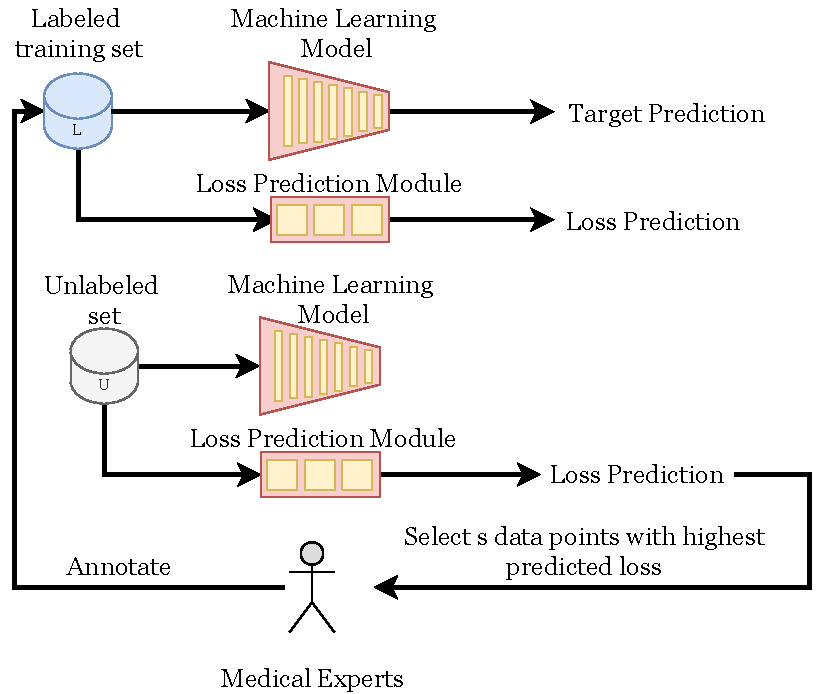
\includegraphics[keepaspectratio,width=0.75\textwidth]{figures/fig_learning_loss_for_active_learning.pdf}
\caption{The labeled set $\mathcal{L}$ is used for training the model for predicting a class for each data point as well as predicting its loss. The trained model is then used for predicting losses of data points in the unlabeled set $\mathcal{U}$. The s data points with the highest loss are selected for annotation by the experts.}
\label{fig:learning_loss_for_active_learning}
\end{figure}

The loss objective function, $L_{loss}(\hat{l}, l)$, has to be chosen such that the scale of the true loss, which decrease as the training progresses, does not impact the overall value of $L_{loss}$. The authors suggest a pairwise loss function. Considering a mini-batch of size $B$, $B/2$ pairs can be obtained: $\{x^p = (x_i, x_j)\}$ and by directly comparing the difference in true and predicted loss for each pair, the decreasing scale of the loss can be discarded. The loss objective function is defined as:
\begin{equation}
    \label{equation:learning_loss_pair_wise_loss}
    L_{loss}(\hat{l}^{p}, l^{p}) = max [0, \mathbb{1}(l_i, l_j)\cdot(\hat{l_i}, \hat{l_j}) + \epsilon ]
\end{equation}
where,
\begin{itemize}[label={}]
  \setlength\itemsep{0em}
  \item $\mathbb{1}$ is the indicator function, $\mathbb{1}(l_i, l_j) = \begin{cases} 
      +1 & if \quad l_i > l_j \\
      -1 & otherwise \\
   \end{cases}$
   \item $\epsilon$ is the predefined positive margin
\end{itemize}

As shown in figure \ref{fig:learning_loss_for_active_learning}, s data points with the highest predicted loss are selected for annotation.

\subsection{Dropout as a Bayesian Approximation: Representing Model Uncertainty in Deep Learning (MC dropout)}
Dropout\cite{srivastava2014} is a commonly used technique for model regularization, which randomly ignores a fraction of neurons during training to mitigate the problem of overfitting. It is typically disabled during test time. MC-dropout involves the assessment of uncertainty in neural networks using dropout at test time \cite{gal2016, gal2016phd} and thus estimates the uncertainty of the prediction of an image. MC-dropout generates non-deterministic prediction distributions for each image. The variance of this distribution can be used as an approximation for model uncertainty $\delta$. During each active learning iteration, the images with the highest variance are annotated and added to $\mathcal{L}$. This has been shown to be an effective selection criterion during active learning \cite{gal2016}. \\
In order to derive the theory which enables the modeling of uncertainty in neural networks using dropout, lets start with some background information by explaining Bayesian modelling and Variational Inference. Let $\mathcal{L} = \{(x_1, y_1), (x_2, y_2), (x_3, y_3) ... ((x_N, y_N))\}$ with $|L| = N$, be a set of labeled data points. The objective is to find the parameters $\Theta$ of a function $f^\Theta$, which map the inputs to outputs i.e. $\hat{Y} = f^\Theta(\mathcal{L})$. The parameters $\Theta$ can be optimized using techniques such as stochastic gradient descent to obtain a single set of $\Theta$, which in turn outputs a single set of predictions $\hat{Y}$. However, in a Bayesian setting, the model is represented as a distribution over the parameters $\Theta$ and hence a predictive posterior distribution over $\hat{Y}$ is obtained. Marginalization is a fundamental part of Bayesian modelling. The marginal likelihood represents an weighted average over the distribution of parameters $\Theta$, weighted by the prior probability $P(\Theta)$. It is formulated as:
\begin{equation}
    \label{equation:marginal_likelihood_mc_dropout}
    P(Y | X) = \int P(Y | X, \Theta) p(\Theta) d\Theta
\end{equation}

Using equation \ref{equation:marginal_likelihood_mc_dropout}, the posterior distribution of parameters $\Theta$ can be formulated using Bayes' Theorem as:
\begin{equation}
    \label{equation:post_dist_theta_mc_dropout}
    P(\Theta | X, Y) = \frac{P(Y | X, \Theta) P (\Theta)}{P(Y | X)}
\end{equation}

where,
\begin{itemize}[label={}]
  \setlength\itemsep{0em}
  \item $P (\Theta)$ is the prior probability over the parameters
\end{itemize}
Using equation \ref{equation:post_dist_theta_mc_dropout}, the label $w_i$ for an unlabeled data point $u_i$ where $(u_i\in\mathcal{U})$ can be predicted as:

\begin{equation}
    \label{equation:prediction_mc_dropout}
    P(w_i | u_i, X, Y) = \int P(w_i|u_i, \Theta)P(\Theta|X, Y)d\Theta
\end{equation}
The process in equation \ref{equation:prediction_mc_dropout} is called Bayesian inference. However, the integral in $P(Y|X)$ can only be calculated analytically for very small datasets. In order to tackle this issue, Variational Inference can be used. \\
The main idea behind Variational Inference is that, as $P(\Theta | X, Y)$ cannot be calculated analytically, a variational distribution $q_\theta$ with parameters $\theta$ can be specified as an approximation of $P(\Theta | X, Y)$. The variational distribution $q_\theta$ is easy to evaluate, so Kullback–Leibler (KL) divergence\cite{kullback1951} is used to optimize the parameters $\theta$ such that $q_\theta$ is as close as possible to $P(\Theta | X, Y)$. KL divergence is formulated as:

\begin{equation}
    \label{equation:kl_divergence_mc_dropout}
    KL(q_\theta(\Theta)|P(\Theta| X, Y)) = \int{q_\theta(\Theta)log\frac{q_\theta(\Theta)}{P(\Theta| X, Y)}d\Theta}
\end{equation}
Replacing $P(\Theta| X, Y)$ with $q_\theta(\Theta)$ in equation \ref{equation:prediction_mc_dropout}:
\begin{equation}
    \label{equation:prediction_replaced_mc_dropout}
    P(w_i | u_i, X, Y) = \int P(w_i|u_i, \Theta)q_\theta(\Theta)d\Theta
\end{equation}
As equation \ref{equation:kl_divergence_mc_dropout} contains $P(\Theta| X, Y)$, it cannot be calculated. However, it has been found that minimizing equation \ref{equation:kl_divergence_mc_dropout} can be done by maximizing evidence lower bound (ELBO)\cite{bishop2006}:
\begin{equation}
    \label{equation:evidence_lower_bound_mc_dropout}
    \mathcal{L}_{VI}(\theta) = \int{q_\theta(\Theta)logP(\Theta| X, Y)d\Theta - KL(q_\theta(\Theta)|P(\Theta))}
\end{equation}

Calculating equation \ref{equation:evidence_lower_bound_mc_dropout} is not computationally tractable for large datasets or complicated approximated distributions. The authors in this paper provide another way to perform Variational Inference, which is scalable and computationally tractable. The approximating distribution is reformulated as $q_{\theta}(\Theta)$ with $\Theta = M_i . diag([Z_{i, j}]_{j=1}^{K_i})$, $Z_i,j \sim Bernoulli(p_i)$ for $i = 1, ...,L$ and $j = 1, ...,K$ and $M_i$ be the weight matrix before dropout. Here, L is the number of layers and K is the number of nodes in each layer. Each $Z_{i,j}$ is Bernoulli random variable which specifies if the input should be set to zero or not with a probability $p_i$. \\
Using the reformulated $q_{\theta}(\Theta)$, it is not possible to calculate equation \ref{equation:evidence_lower_bound_mc_dropout} because of the integral. Two ways in which this problem is tackled are:
\begin{itemize}
  \setlength\itemsep{0em}
  \item The integral in equation \ref{equation:evidence_lower_bound_mc_dropout} can be approximated using loss functions such as softmax loss and mean squared error loss with L2 regularization.
  \item This variational inference is equivalent to a Gaussian Process (GP) approximation of neural network with model precision $\tau$ and length scale l, meaning we get an approximation of distribution over possible functions by Monte Carlo estimation\cite{raychaudhuri2008} i.e. as shown in figure \ref{fig:mc_dropout}, by repeating the experiment m number of times, here m is also called Monte Carlo iterations.
\end{itemize}
The posterior distribution of parameters $\Theta$ can now be approximated along with the mean and variance. Thus, the uncertainty values obtained through MC dropout can be used for active learning.

\begin{figure}[htbp]
\centering
\captionsetup{format=plain}
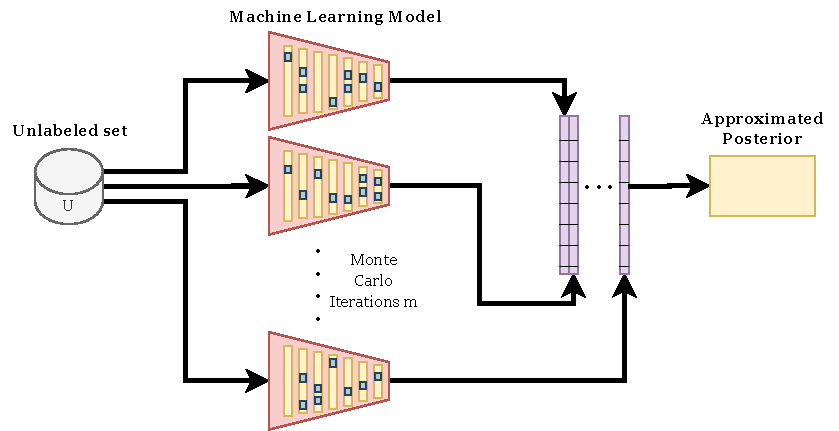
\includegraphics[keepaspectratio,width=0.95\textwidth]{figures/fig_mc_dropout.pdf}
\caption{During each Monte Carlo iteration, dropout disables certain units in the neural network. This results in a different version of the same model during each iteration. Unlabeled dataset is passed through the modified versions of the model m times. Using the predictions obtained from the m Monte Carlo iterations, the posterior distribution can be approximated.}
\label{fig:mc_dropout}
\end{figure}

\subsection{Augmentations-based sampling}
Let $\mathcal{A}$ be a function which performs stochastic data augmentations such as cropping, horizontal flipping, vertical flipping or erasing in case of an image (further details on $\mathcal{A}$ are provided in appendix). Each unlabeled data point $u_i\in\mathcal{U}$, is transformed using $\mathcal{A}$ and this process is repeated J times, to obtain $U_i = \{u_{1i}^{`}, u_{2i}^{`}, u^{`}_{3i}, ... u_{Ji}^{`}\}$. The random transformations are followed by a forward pass through the model $f^\Theta$ with parameters $\Theta$, which results in N predictions $\hat{Q}_i = \{\hat{q}_{1i}, \hat{q}_{2i}, \hat{q}_{3i} ... \hat{q}_{Ni}\}$ where $\hat{q}_i = argmax(P_\Theta(\hat{y}_i|x_i)$ is the most probable class according to the model output, for each set of perturbed copies of a unlabeled data point $U_i$. An uncertainty measure based on the mode of J predictions, introduced in this paper\cite{sadafi2019} is used for labeling the data points that the model is most uncertain about. The proposed uncertainty measure is:

\begin{equation}
    \label{equation:augmentation_based_sampling}
    \delta_{i} = \frac{1}{J} \sum_{k=1}^{J} \mathbb{1}(\hat{q}_{ik}, M(\hat{Q}_i))
\end{equation}

where,
\begin{itemize}[label={}]
  \setlength\itemsep{0em}
  \item $\delta_{i}$ represents the uncertainty measure of the $i^{th}$ data point
  \item J is the size of $U_i$ i.e. $|U_i| = J$
  \item $\hat{q}_{ik}$ represents the prediction for the $k^{th}$ element of $U_i$
  \item $M(\hat{Q}_i)$ represents the mode of $\hat{Q}_i$
  \item $\mathbb{1}$ is the indicator function, $\mathbb{1}(\hat{y}_{ik}, M(\hat{Q}_i)) = \begin{cases} 
      1 & if \quad \hat{y}_{ik} \neq M(\hat{Q}_i) \\
      0 & otherwise \\
   \end{cases}$
\end{itemize}

Hence, The model uncertainty $\delta$ can be estimated by keeping a count of the most frequently predicted class (mode) for each image. The idea behind this approach is that if the model is certain about an image then it should output the same prediction for randomly augmented versions. So the lower the frequency of the mode, the higher the uncertainty $\delta$ \cite{sadafi2019}. During each active learning iteration, the images with  the lowest frequency of the most frequently predicted class are annotated and added to $\mathcal{L}$.

\begin{figure}[htbp]
\centering
\captionsetup{format=plain}
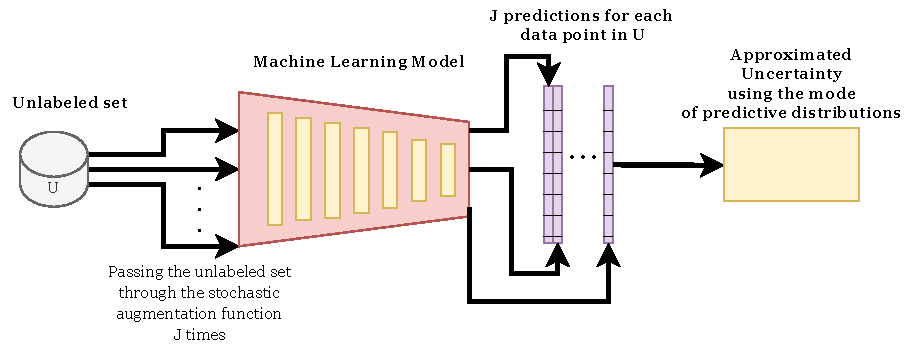
\includegraphics[keepaspectratio,width=0.95\textwidth]{figures/fig_augmentations_based.pdf}
\caption{Each data point in $\mathcal{U}$ is passed through the stochastic augmentation function $\mathcal{A}$, J times to obtain J predictive distributions for each data point. The model uncertainty $\delta$ is estimated by taking a mode of the predictive distributions.}
\label{fig:augmentations_based}
\end{figure}

\section{Pre-training Methods}\label{section:pretraining_methods}
Network initialization can increase the performance of neural networks \cite{hanin2018}. It is considered to be even more essential when the amount of annotated data is not considerably large \cite{holmberg2020}. In this thesis I utilize three different pre-training methods plus random initialization (baseline):

\subsection{Random initialization}
Random initialization was shown to perform poorly compared to more sophisticated initialization measures \cite{glorot2010}. Kaiming He initialization \cite{he2015} is used as a baseline random initialization method. Kaiming He initialization, takes asymmetric activation function such as ReLU into account while weights initialization. It is shown\cite{he2015}, that the initialization methods, such as xavier initialization\cite{glorot2010} and Gaussian initialization, which do not take the asymmetric nature of activation function into account suffer from exploding or vanishing gradients problem. Consider forward propagation through a Neural Network:

\begin{equation}
    \label{equation:forward_pass}
    Y_l = W_lX_l + B_l
\end{equation}

where,
\begin{itemize}[label={}]
  \setlength\itemsep{0em}
  \item $l$ is the layer
  \item $Y_l$ is the output of layer l before it goes through the activation function
  \item $W_l$ is the weights matrix. The initialized elements in $W_l$ share the same distribution and are mutually independent
  \item $X_l$ is the output of previous layer after it goes through the activation function i.e. $X_l = f(Y_{l-1})$. The elements in $X_l$ share the same distribution and are mutually independent
  \item $B_l$ is the bias vector
  \item $W_l$ and $X_l$ are mutually independent of each other
\end{itemize}

Taking variance of equation \ref{equation:forward_pass}, we get:

\begin{equation}
    \label{equation:variance_forward_pass}
    Var[y_l] = n_l Var[w_lx_l]
\end{equation}

where,
\begin{itemize}[label={}]
  \setlength\itemsep{0em}
  \item $n_l$ is the number of activations in layer l
  \item $y_l$, $w_l$ and $x_l$ are the random variables of $Y_l$, $W_l$ and $X_l$ respectively
\end{itemize}

Assuming that the random variable $w_l$ has zero mean, we can further simplify equation \ref{equation:variance_forward_pass}:

\begin{equation}
    \label{equation:expectation_forward_pass}
    Var[y_l] = n_l Var[w_l]\mathbf{E}[x_l^2]
\end{equation}

where,
\begin{itemize}[label={}]
  \setlength\itemsep{0em}
  \item $\mathbf{E}$ refers to the expectation
\end{itemize}

Consider the ReLU activation i.e. $x_l = max(0, y_{l-1})$. If we let $w_{l-1}$ have a symmetric distribution around zero and $b_{l-1} = 0$ then $y_{l-1}$ will also be symmetric around zero and will have zero mean. This leads to $\mathbf{E}[x_l^2] = \frac{1}{2}Var[y_{l-1}]$, when the activation function is ReLU. Replacing the value of $\mathbf{E}[x_l^2]$ in equation \ref{equation:expectation_forward_pass}, we get:

\begin{equation}
    \label{equation:replaced_expectation_forward_pass}
    Var[y_l] = \frac{1}{2}n_l Var[w_l]Var[y_{l-1}]
\end{equation}

Now we have a recurrence relation between the activations of layer l and l-1. So starting from the last layer O and continuing on till the first one, we get:

\begin{equation}
    \label{equation:final_layers_forward_pass}
    Var[y_O] = Var[y_1] \left( \prod_{l=2}^{O} \frac{1}{2}n_l Var[w_l] \right)
\end{equation}

Hence, for a large number of layers, we see that if $\frac{1}{2}n_l Var[w_l]$ is greater than 1, then variance at the last layer O can be very large and if $\frac{1}{2}n_l Var[w_l]$ is less than 1, then the variance at the last layer O can be very small. Kaiming He initialization, aims to keep $\frac{1}{2}n_l Var[w_l] = 1$. To achieve this, Kaiming He initialization sets the weights of layer l to a zero-mean Gaussian distribution with a standard deviation of $\sqrt{\frac{2}{n_l}}$ and null biases.

\subsection{ImageNet Weights}
ImageNet weights are obtained by training a feature extraction network on the ImageNet dataset. After training on ImageNet data, the weights of the feature extractor network can be used for initialization of models which are to be trained on other datasets \cite{raghu2019}. This has become a standard pre-training for classification tasks as it often helps the network converge faster than with random initialization. It also has been shown to be beneficial in low-data biomedical imaging regimes \cite{raghu2019}. 

\subsection{Autoencoder}
Traditional autoencoders\cite{kramer1991} are the most prominent example of neural networks used for feature extraction. The objective of the autoencoders is to reconstruct the input. 

\begin{figure}[htbp]
\centering
\captionsetup{format=plain}
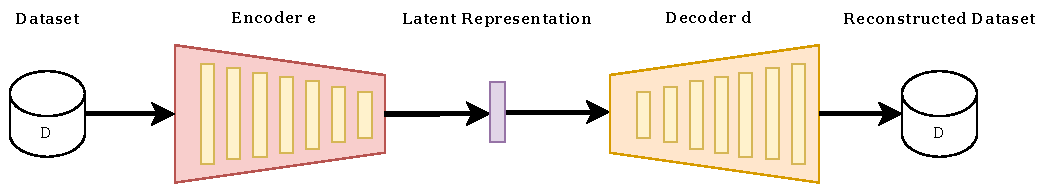
\includegraphics[keepaspectratio,width=\textwidth]{figures/fig_autoencoder.pdf}
\caption{The encoder e consists of convolutional layers, which iteratively downsample the input into a latent representation. The decoder d consists of transposed convolutional layers, which iteratively upsample the input. The goal of the autoencoder is to encoder the input into latent space and then reconstruct it.}
\label{fig:autoencoder}
\end{figure}

As shown in the figure \ref{fig:autoencoder}, the autoencoder consists of an encoder and a decoder network. The encoder network $f^{\Theta_{enc}}$ with parameters $\Theta_{enc}$, encodes the input ($u_i$) into a compact form i.e. $h_i = f^{\Theta_{enc}}(u_i)$. The compression is carried out by a bottleneck layer, which contains relatively few nodes. The bottleneck layer forces the encoder to represent the input data in a compact form. This compact form is called a latent representation and it is used as an input to a decoder network $f^{\Theta_{dec}}$ with parameters $\Theta_{dec}$, which tries to output a reconstruction $f^{\Theta_{dec}}(f^{\Theta_{enc}}(u_i))$, of the original input. \\
The autoencoders try to find a lower dimensional encoding of the input data. They are widely used for dimensionality reduction. Principal Component Analysis (PCA), is another dimensionality reduction technique which is restricted to linear maps. A linear autoencoder without any non-linear activation functions, spans the same subspace as PCA\cite{baldi1989}. Autoencoders work on the basis of the assumption that there are underlying substructures within the data which can be represented in the latent representation and they can be trained in an unsupervised manner. This allows the autoencoders to be used for pre-training.
The objective function of autoencoders can be stated as:
\begin{equation}
    \label{equation:autoencoders_loss}
    Loss = \sum_{i}^{K} \left\Vert u_i - f^{\Theta_{dec}}(f^{\Theta_{enc}}(u_i)) \right\Vert^2
\end{equation}

where,
\begin{itemize}[label={}]
  \setlength\itemsep{0em}
  \item $f^{\Theta_{enc}}$ is the encoder network
  \item $f^{\Theta_{dec}}$ is the decoder network
  \item K is the length of $\mathcal{U}$
\end{itemize}

Hence autoencoders do not require labels for training and the whole dataset can be used for training an autoencoder architecture. For pre-training the encoder is used as a feature extraction network while the decoder is generally discarded. This has been shown to significantly improve network initialization on biomedical image datasets \cite{ferreira2020}.

\subsection{A Simple Framework for Contrastive Learning of Visual Representations}
A Simple Framework for Contrastive Learning of Visual Representations (SimCLR), is a framework for contrastive learning of visual representations \cite{chen2020}. As shown in figure \ref{fig:simclr}, it learns representations in a self-supervised manner by using an objective function that minimizes the difference between representations of the model $f^{\Theta}$ with parameters $\Theta$ on a pairs of differently augmented copies of the same data point. \\
Let $\mathcal{A}$ be a function which performs stochastic data augmentations (such as cropping, adding color jitter, horizontal flipping and gray scale) on a given data point. Each data point $x, \forall x \in \mathcal{D}$ in a mini-batch of size $\mathcal{B}$, is passed through the stochastic data augmentations function $\mathcal{A}$ twice, to obtain $X_i = \{x_{1i}^{`}, x_{2i}^{`}\}$ with $\forall x_i^{`} \in X_i = \mathcal{A}(x_i)$. These pairs can be termed as positive pairs as they originate from the same data point. A neural network encoder ($f^{\Theta_{enc}}$ with parameters $\Theta_{enc}$), extracts the feature vectors from the augmented data points:

\begin{equation}
    \label{equation:simclr_encoder}
    h_k = f^{\Theta_{enc}}(x_k)
\end{equation}

where,
\begin{itemize}[label={}]
  \setlength\itemsep{0em}
  \item $h_k \in \mathbb{R}^{d}$ is the feature vector for $k^{th}$ data point
\end{itemize}

A multi-layer perceptron ($f^{\Theta_{MLP}}$ with parameters $\Theta_{MLP}$) with one hidden layer is used as a projection head for projecting the feature vectors h to projection space where the contrastive loss is applied. It is shown\cite{chen2020} that applying contrastive loss in projection space is better than applying it in the feature space. The projections are obtained by:

\begin{equation}
    \label{equation:simclr_mlp}
    z_k = f^{\Theta_{MLP}}(h_k) = W^{2}\sigma(W^{1}h_k)
\end{equation}

where,
\begin{itemize}[label={}]
  \setlength\itemsep{0em}
  \item $z_k \in \mathbb{R}^{p}$ is the projection $k^{th}$ feature vector
  \item $h_k \in \mathbb{R}^{d}$ is the feature vector for $k^{th}$ data point
  \item $\sigma$ is the ReLU\cite{nwankpa2018} non-linear activation function
\end{itemize}
After performing stochastic augmentations on each data point in a mini-batch of size $\mathcal{B}$, the total number of data points increase to $2\mathcal{B}$. This results in $\mathcal{B}$ positive pairs and $2(\mathcal{B}-1)$ negative pairs (which can be obtained by pairing up an augmented data point with any other data point in the set except its own second augmented version). The contrastive loss for a positive pair $(x_{1i}^{`}, x_{2i}^{`})$ can be termed as:

\begin{equation}
    \label{equation:simclr_contrastive_loss}
    L_{(1i, 2i)} = -log \frac{exp(sim(z_{1i}, z_{2i}) / \tau)}{\sum_{k=1}^{2\mathcal{B}} \mathbb{1}[k\neq 1i] exp(sim(z_{1i}, z_{k}) / \tau)}
\end{equation}

where,
\begin{itemize}[label={}]
  \setlength\itemsep{0em}
  \item $\mathbb{1}$ is the indicator function, $\mathbb{1}(k, 1i) = \begin{cases} 
      1 & if \quad k \neq 1i \\
      0 & otherwise \\
   \end{cases}$ 
   \item $\tau$ denotes a temperature parameter. 
   \item $sim(x, y)$ is the cosine similarity function: $sim(x, y) = \frac{x^{T}y}{||x||||y||}$
   \item The final loss value is obtained by computing it across all positive pairs i.e. (1i, 2i) and (2i, 1i).
\end{itemize}

\begin{figure}[htbp]
\centering
\captionsetup{format=plain}
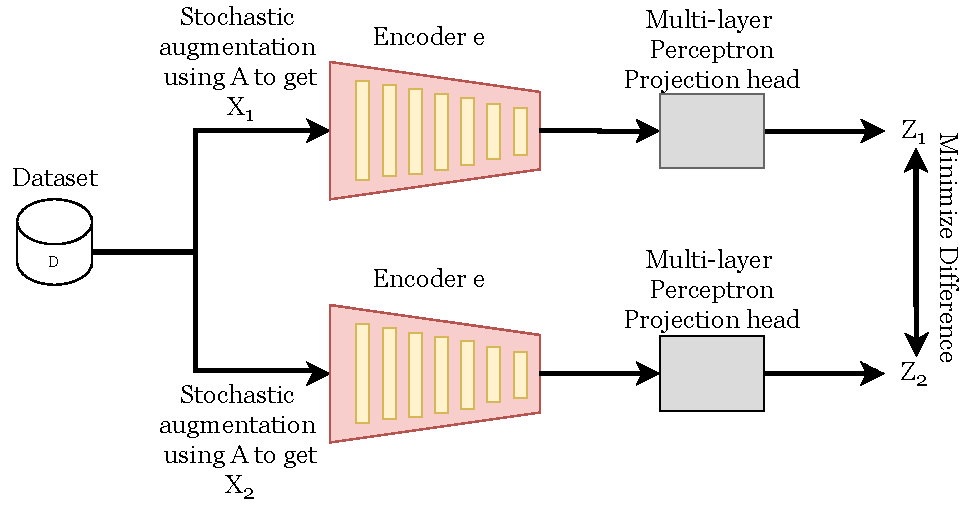
\includegraphics[keepaspectratio,width=\textwidth]{figures/fig_simclr.pdf}
\caption{The whole dataset $\mathcal{D}$, is passed through a stochastic augmentation function $\mathcal{A}$ to get $X_1$ and $X_2$. The augmented data points are passed through the model to get feature vector. A projection head projects the feature vectors to $Z_1$ and $Z_2$, where the contrastive loss is applied.}
\label{fig:simclr}
\end{figure}


\section{Training strategies}\label{section:training_strategies}
Large amounts of unlabeled data are typically available in biomedical applications. Ideally, this unlabeled data is not only used for network initialization but also during training. Thus, the performance of training the model is compared by using only the existing labeled data a.k.a. supervised learning versus a semi-supervised approach which incorporates the unlabeled data in the training process.

\subsection{Supervised Learning}
In supervised learning we are looking for a model $f^\Theta$ with parameters $\Theta$ to learn a mapping $\hat{Y} = f^\Theta(\mathcal{L})$ such that the objective function Loss $(\hat{y}_i, y_i)$ is minimized. Supervised learning uses only labeled data. The performance of the model can be evaluated using an evaluation metric $\mathcal{M}$ such as accuracy, recall etc. The objective function used in this paper is the multi-class cross-entropy loss function, $Loss = - \sum_{i}^{N} \sum_{j}^{C} y_{ij}log(\hat{y}_{ij})$ with C being the total number of classes in the dataset and N being the size of $\mathcal{L}$.


\subsection{Pseudo-Labeling}
Pseudo Labeling is considered to be a Wrapper method. Wrapper methods are one of the oldest known semi-supervised learning techniques\cite{van2020}. Wrapper methods involve training a base learner with $\mathcal{L}$ as well as $\mathcal{U}$, for which the labels are acquired through pseudo-labeling\cite{mclachlan1975}. The training process involves two steps: the base learner is trained on $\mathcal{L}$ as well as the pseudo-labeled set from previous iterations and then predictions ($\hat{y}$) are obtained on $\mathcal{U}$. The unlabeled data points ($x \in \mathcal{U}$), for which the base learner outputs predictions with a high confidence are assigned the corresponding predicted label and added to training set as pseudo-labeled data for the next iteration. \\
An advantage of wrapper methods is that, they can be added as a wrapper around the base learner. The base learner doesn't have to be modified and the pseudo-labeled data is processed as normal labeled data by the base learner.

\subsection{FixMatch: Simplifying Semi-Supervised Learning with Consistency and Confidence}
As shown in figure \ref{fig:fixmatch}, FixMatch\cite{sohn2020} is a combination of two approaches in semi-supervised learning: consistency regularization\cite{sajjadi2016} and pseudo labeling\cite{mclachlan1975}. The main contribution of the authors is the combination of both concepts and using strong and weak augmentations for consistency regularization (for further details about the strong and weak augmentations, please refer to the FixMatch paper). \\
Given the set of unlabeled data points $\mathcal{U} = \{u_1, u_2, u_3 ... u_K\}$ with $|U| = K$, consistency regularization tries to maximize the similarity between model ($f^\Theta$ with parameters $\Theta$) outputs, obtained by passing stochastically augmented versions of the same data point. \\
Pseudo labeling refers to using artificial labels for unlabeled data points. The artificial labels are obtained by passing the unlabeled data points through the model $f^\Theta$) i.e. $\hat{Y} = f^\Theta(\mathcal{U}$ and using the outcome $q$ with maximum probability in the predicted distribution i.e. $q_i = argmax(P_{\Theta}(y_i | x_i))$ as the artificial label, if the maximum probability value is above a threshold $\tau$. Using the artificial labels, the unlabeled data points are added to the set of labeled data points $\mathcal{L}$. Pseudo labeling uses the following loss function on the unlabeled data points:
\begin{equation}
    \label{equation:fixmatch_pseudo_labeling_loss}
    L_{pseudo} = \frac{1}{K} \sum_{k=0}^{K} \mathbb{1}(max(P_{\Theta}(y_i | x_i)) \geq \tau) H(P_{\Theta}(\hat{y}_i | x_i), P_{\Theta}(y_i | x_i))
\end{equation}

where,
\begin{itemize}[label={}]
  \setlength\itemsep{0em}
  \item K is the size of unlabeled dataset $\mathcal{U}$
  \item $\mathbb{1}$ is the indicator function, $\mathbb{1}(max(P_{\Theta}(y_i | x_i) \geq \tau) = \begin{cases} 
      1 & if \quad max(P_{\Theta}(y_i | x_i) \geq \tau \\
      0 & otherwise \\
   \end{cases}$ 
   \item $\tau$ denotes the pseudo labeling threshold 
   \item H is the cross entropy loss function
\end{itemize}
Consider two stochastic augmentations functions: the weak augmentations function $\alpha$ and strong augmentations function $\mathcal{A}$. The objective function in the FixMatch paper is comprised of two loss terms, the supervised loss term $L_{supervised}$ and unsupervised loss term $L_{unsupervised}$. The complete objective function is formulated as:
\begin{equation}
    \label{equation:fixmatch_loss}
    L_{pseudo} = L_{supervised} + \lambda L_{unsupervised}
\end{equation}

where,
\begin{itemize}[label={}]
  \setlength\itemsep{0em}
  \item $\lambda$ is the weighting factor for the unsupervised loss term
\end{itemize}

The supervised loss is simply the cross entropy loss on the weakly augmented examples within $\mathcal{L}$. $L_{supervised}$ is formulated as:

\begin{equation}
    \label{equation:fixmatch_supervised_loss}
    L_{supervised} = \frac{1}{N} \sum_{i=0}^{N} H(P_{\Theta}(\hat{y}_i | x_i), P_{\Theta}(y_i | x_i))
\end{equation}

where,
\begin{itemize}[label={}]
  \setlength\itemsep{0em}
  \item N is the size of the labeled dataset $\mathcal{L}$
  \item $P_{\Theta}(\hat{y}_i | x_i)$ is the predicted distribution
  \item $P_{\Theta}(y_i | x_i)$ is the ground truth distribution
\end{itemize}

For the unsupervised loss, the unlabeled dataset $\mathcal{U}$, is passed through the stochastic weak augmentation function $\alpha$ and then pseudo labeling is applied on the output prediction distribution with threshold $\tau$. Consistency regularization is applied by calculating cross entropy between the pseudo labels and the labels obtained after passing the points through the strong augmentation function $\mathcal{A}$. $L_{unsupervised}$ is formulated as:

\begin{equation}
    \label{equation:fixmatch_unsupervised_loss}
    L_{unsupervised} = \frac{1}{K} \sum_{k=0}^{K} \mathbb{1}(max(P_{\Theta}(y_i | x_i)) \geq \tau) H(P_{\Theta}(\hat{y}_i | \mathcal{A}(x_i)), P_{\Theta}(y_i | x_i))
\end{equation}

where,
\begin{itemize}[label={}]
  \setlength\itemsep{0em}
  \item K is the size of unlabeled dataset $\mathcal{U}$
  \item $\mathbb{1}$ is the indicator function, $\mathbb{1}(max(P_{\Theta}(y_i | x_i) \geq \tau) = \begin{cases} 
      1 & if \quad max(P_{\Theta}(y_i | x_i) \geq \tau \\
      0 & otherwise \\
   \end{cases}$ 
   \item $\tau$ denotes the pseudo labeling threshold 
   \item H is the cross entropy loss function
   \item $P_{\Theta}(y_i | x_i)$ is the distribution obtained after pseudo labeling
   \item $P_{\Theta}(\hat{y}_i | \mathcal{A}(x_i))$ is the predicted distribution after strong augmentation
\end{itemize}

\begin{figure}[htbp]
\centering
\captionsetup{format=plain}
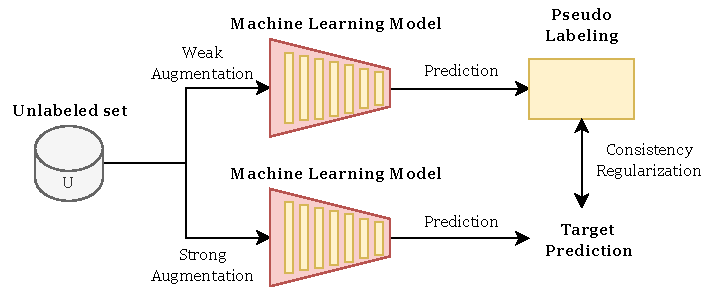
\includegraphics[keepaspectratio,width=0.85\textwidth]{figures/fig_fixmatch.pdf}
\caption{Each data point in the unlabeled set $\mathcal{U}$, is passed through a weak augmentation function and a strong augmentation function, $\alpha$ and $\mathcal{A}$ respectively. Pseudo labeling is applied on the prediction output of weakly augmented data points. Consistency regularization is carried out with the prediction output of strongly augmented data points and the pseudo labeled weakly augmented data points. The consistency regularization gives us the unsupervised loss term.}
\label{fig:fixmatch}
\end{figure}
